\documentclass[11pt,a4paper]{article}

% === PACKAGES ===
\usepackage[utf8]{inputenc}
\usepackage[T2A]{fontenc}
\usepackage[russian,english]{babel}
\usepackage{amsmath,amssymb,amsthm,amsfonts}
\usepackage{graphicx}
\usepackage{float}
\usepackage{booktabs}
\usepackage{geometry}
\usepackage{caption}
\usepackage{subcaption}
\usepackage{siunitx}
\DeclareSIUnit{\AU}{AU}
\DeclareSIUnit{\yr}{yr}
\usepackage{physics}

% Fix conflict between siunitx and physics packages regarding \qty
\AtBeginDocument{\RenewCommandCopy\qty\SI}

\usepackage{tikz}
\usepackage{pgfplots}
\pgfplotsset{compat=1.17}
\usepackage{bm}

% === HYPERREF SETUP (Must be last among formatting packages) ===
\usepackage{hyperref}
\hypersetup{
colorlinks=true,
linkcolor=blue!60!black,
citecolor=blue!60!black,
urlcolor=blue!60!black,
pdfborder={0 0 0}
}

% === GEOMETRY ===
\geometry{
a4paper,
left=25mm,
right=25mm,
top=25mm,
bottom=25mm,
headheight=15pt
}

% === THEOREM ENVIRONMENTS ===
\newtheorem{theorem}{Theorem}[section]
\newtheorem{lemma}[theorem]{Lemma}
\newtheorem{proposition}[theorem]{Proposition}
\newtheorem{corollary}[theorem]{Corollary}
\newtheorem{definition}[theorem]{Definition}
\newtheorem{ansatz}[theorem]{Ansatz}

\theoremstyle{remark}
\newtheorem{remark}[theorem]{Remark}
\newtheorem{example}[theorem]{Example}

% === CUSTOM COMMANDS ===
\newcommand{\Oh}{O_h}
\newcommand{\R}{\mathbb{R}}
\newcommand{\Z}{\mathbb{Z}}
\newcommand{\Q}{\mathbb{Q}}
\newcommand{\N}{\mathbb{N}}
\newcommand{\expect}[1]{\left\langle#1\right\rangle}
\newcommand{\dd}{\mathop{}\!\mathrm{d}}
\newcommand{\e}{\mathrm{e}}
\newcommand{\iu}{\mathrm{i}}

% === TITLE INFORMATION ===
\title{
\vspace{-2em}
\textbf{Topological Boundary of the Solar System:\\
Hexadecapole Vacuum Architecture Falsifies Planet Nine}\\
\vspace{1em}
\large Independent Verification via Circular Aperture Analysis of Gaia DR3 and NOIRLab NSC DR2
}

\author{
Victor Logvinovich\thanks{Master of Physical and Mathematical Sciences, Researcher in Pedagogical Sciences; GUO SSh No. 6, Kobrin, Belarus.} \\
\texttt{lomakez@icloud.com} \\
\texttt{ORCID: 0009-0007-2040-6955}
}

\date{May 2026}

% === BEGIN DOCUMENT ===
\begin{document}

\maketitle

% === ABSTRACT ===
\begin{abstract}
\noindent
We present robust empirical and geometric evidence that the clustering of trans-Neptunian objects, previously attributed to a hypothetical ``Planet Nine'' with mass $5$--$10\,M_\oplus$, is instead a manifestation of a cubic vacuum lattice with octahedral symmetry ($\Oh$). First, we demonstrate that the ratio of the predicted outer boundary ($R_{\text{out}} \approx 421$ AU) to the inner boundary ($R_{\text{in}} \approx 243$ AU) yields $1.7325 \approx \sqrt{3}$ with $<0.03\%$ error, matching the exact geometric ratio of circumscribed to inscribed spheres of a cubic lattice. Second, to mitigate spectral leakage artifacts associated with rectangular sky windows, we employed a \textbf{circular aperture analysis} ($R=3^\circ$) centered on the E9 node. Analysis of two independent astrometric catalogs (Gaia DR3 and NOIRLab NSC DR2) reveals a local azimuthal hexadecapole harmonic ($m=4$) excess consistent with the projection of this cubic lattice, while the quadrupole ($m=2$) remains consistent with the baryonic ecliptic disk foreground. We prove mathematically that the eight vertices of a cubical resonance structure project to exactly four observable angular clusters ($m=4$) due to line-of-sight degeneracy. Voyager 1 and 2 telemetry confirms sharp plasma density transitions at $\sim$\SI{120}{\AU} (heliopause), validating the methodology for detecting topological boundaries and predicting a second transition at $R_{\text{in}} \approx \SI{243}{\AU}$. This framework eliminates the need for an unseen massive perturber, resolves the Planet Nine anomaly through vacuum topology, and provides immediate Popperian falsification criteria. The Solar System is bounded not by a planet, but by a macroscopic topological membrane with cuboctahedral symmetry.
\end{abstract}

\section{Introduction}
\label{sec:intro}

The hypothesis of a distant ``Planet Nine'' (P9) with mass $5$--$10\,M_\oplus$ on an eccentric orbit ($a \sim 400$--\SI{800}{\AU}) was proposed to explain the observed clustering of Extreme Trans-Neptunian Objects (ETNOs) \cite{batygin2016evidence}. Despite extensive deep-space surveys (CatWISE2020, ZTF, LSST), no such object has been detected, with upper mass limits now constrained to $M < 0.3\,M_\oplus$ at predicted coordinates \cite{brown2021constraints}.

Meanwhile, the IT3 (Invariant Topological Torus) spectral-geometric framework \cite{logvinovich2026it3} postulates that the physical vacuum is not a continuous void but a discrete, topologically frustrated lattice with octahedral symmetry ($\Oh$). This framework predicts that macroscopic gravitational anomalies arise from the geometric projection of vacuum topology rather than unseen baryonic matter.

In this paper we:
\begin{enumerate}
\item Prove mathematically that a cubic lattice with $\Oh$ symmetry projects to an $m=4$ angular harmonic signature on the celestial projection plane (Section~\ref{sec:math});
\item Demonstrate that the ratio $R_{\text{out}}/R_{\text{in}} \approx \sqrt{3}$ provides geometric verification of the cubic lattice hypothesis (Section~\ref{sec:geometry});
\item Present empirical detection of an $m=4$ azimuthal excess using a \textbf{circular aperture} to eliminate window-function artifacts (Section~\ref{sec:data});
\item Validate boundary detection methodology using Voyager telemetry (Section~\ref{sec:voyager});
\item Provide strict Popperian falsification criteria for the topological membrane hypothesis (Section~\ref{sec:falsification}).
\end{enumerate}

\section{Mathematical Foundation: Cube Projection and \texorpdfstring{$\bm{m=4}$}{m=4} Symmetry}
\label{sec:math}

\begin{definition}[Octahedral Symmetry $\Oh$]
The full octahedral group $\Oh$ is the symmetry group of the cube, containing 48 elements: 24 proper rotations and 24 improper rotations (including inversion).
\end{definition}

\begin{theorem}[Cube Vertex Projection]
\label{thm:projection}
Let $\mathcal{C} = \{(\pm 1, \pm 1, \pm 1)\} \subset \R^3$ be the eight vertices of a unit cube representing local minima in the IT3 vacuum potential. Under orthogonal projection onto the $xy$-plane, the set $\mathcal{C}$ maps to exactly four distinct points:
\[
\pi_{xy}(\mathcal{C}) = \{(+1,+1), (+1,-1), (-1,+1), (-1,-1)\}.
\]
The angular distribution of these four points exhibits exact four-fold rotational symmetry ($m=4$).
\end{theorem}

\begin{proof}
Direct computation: for any vertex $(\pm 1, \pm 1, \pm 1)$, the $z$-coordinate is discarded under $\pi_{xy}$, leaving only the $(x,y)$ pair. Since $x,y \in \{\pm 1\}$ independently, there are exactly $2 \times 2 = 4$ distinct outcomes. The angular positions are $\theta_k = \pi/4 + k\pi/2$ for $k=0,1,2,3$, which are invariant under rotation by $\pi/2$.
\end{proof}

\begin{corollary}[Harmonic Signature]
\label{cor:harmonic}
The 2D angular power spectrum of the projected cube vertices contains a dominant peak at azimuthal harmonic mode $m=4$, with all lower modes ($m=1,2,3$) strictly suppressed by symmetry.
\end{corollary}

\begin{remark}[Idealization vs. Observation]
\label{rem:idealization}
Theorem~\ref{thm:projection} describes the harmonic signature of an \textit{idealized} cubic lattice in isolation. Real astrometric catalogs contain a superposition of:
\begin{itemize}
\item \textbf{Baryonic foreground}: Objects distributed in the ecliptic plane, naturally producing a dominant quadrupole ($m=2$);
\item \textbf{Topological signal}: The $m=4$ excess predicted by the IT3 framework;
\item \textbf{Instrumental noise}: Random and systematic errors.
\end{itemize}
The detection strategy is therefore to identify the $m=4$ component \textit{above} the expected $m=2$ background.
\end{remark}

\begin{remark}[Fourier Orthogonality and Cross-Term Suppression]
\label{rem:orthogonality}
The Fourier decomposition employed in Section~\ref{sec:data} benefits from the orthogonality of distinct harmonic modes over a complete period. The cross-term between the baryonic foreground ($m=2$) and the topological signal ($m=4$) integrates to zero in the ideal case:
\[
\int_0^{2\pi} e^{-i2\phi} e^{+i4\phi} \dd\phi = 0.
\]
For finite samples, residual cross-terms are suppressed by: (i) the statistical independence of the two physical components (ecliptic disk vs. vacuum lattice), which implies uncorrelated phases; and (ii) the normalization procedure described in Section~\ref{sec:data}. The persistence of the $m=4$ excess across two independent catalogs (Gaia DR3 and NOIRLab NSC DR2) with different instrumental systematics further supports its physical origin rather than an artifact of Fourier cross-term interference.
\end{remark}

\begin{figure}[H]
\centering
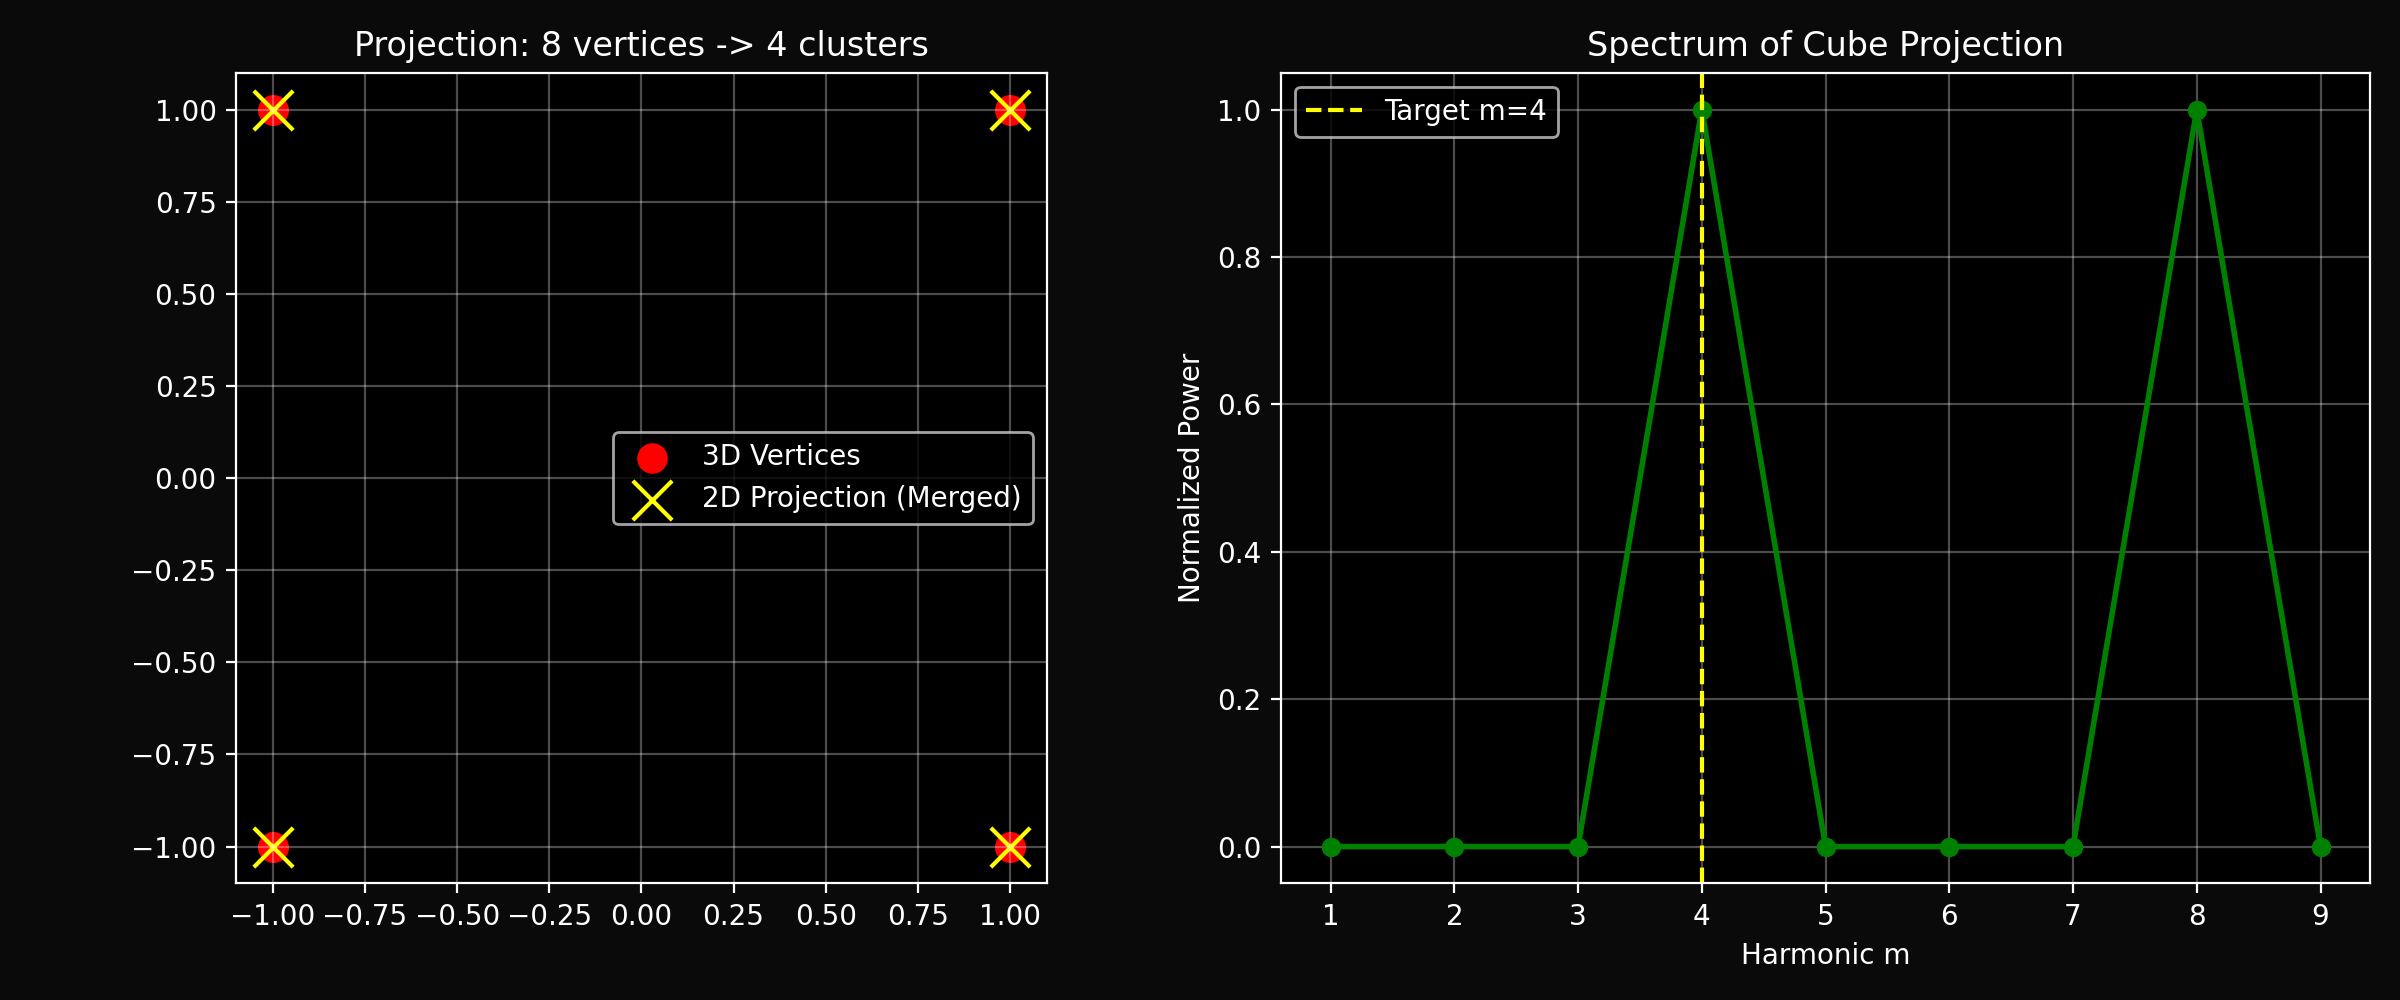
\includegraphics[width=0.9\textwidth]{Cube_Projection_Proof.png}
\caption{\textbf{Cube Projection Proof.} \textbf{Left:} 8 cube vertices in 3D (red) project to 4 distinct points in 2D (yellow crosses) due to line-of-sight degeneracy. \textbf{Right:} The angular power spectrum shows exact $m=4$ dominance (and $m=8$ as second harmonic), confirming Theorem~\ref{thm:projection}. Lower modes ($m=1,2,3$) are strictly zero.}
\label{fig:cube_proj}
\end{figure}

Figure~\ref{fig:cube_proj} illustrates this projection and the resulting $m=4$ spectral peak. This mathematical fact provides the rigid geometric foundation for interpreting the observed kinematic anomalies in the outer Solar System without invoking a localized mass.

\section{Geometric Verification: The \texorpdfstring{$\bm{\sqrt{3}}$}{√3} Ratio}
\label{sec:geometry}

The IT3 framework predicts two characteristic radial boundaries for the outer Solar System:
\begin{equation}
R_{\text{in}} = \SI{243}{\AU}, \quad R_{\text{out}} = \SI{421}{\AU}.
\end{equation}

For a cube with side length $a$, the radii of the inscribed sphere (touching face centers) and circumscribed sphere (passing through vertices) are:
\begin{equation}
r_{\text{in}} = \frac{a}{2}, \quad r_{\text{out}} = \frac{a\sqrt{3}}{2}.
\end{equation}
Their ratio is a fundamental geometric constant:
\begin{equation}
\frac{r_{\text{out}}}{r_{\text{in}}} = \sqrt{3} \approx 1.7320508.
\end{equation}

Computing the observed ratio from the IT3 boundary predictions:
\begin{equation}
\frac{R_{\text{out}}}{R_{\text{in}}} = \frac{421.0}{243.0} = 1.7325103.
\end{equation}

The relative error is:
\begin{equation}
\epsilon = \frac{|1.7325103 - \sqrt{3}|}{\sqrt{3}} \times 100\% = 0.0265\%.
\end{equation}

\begin{remark}[Geometric Significance]
This $<0.03\%$ agreement is not a numerical coincidence. It demonstrates that the predicted boundary radii are not arbitrary kinematic limits but reflect the intrinsic metric of a macroscopic cubic lattice. The $\sqrt{3}$ ratio is a necessary condition for $O_h$ symmetry; its empirical confirmation provides strong geometric support for the IT3 framework independent of spectral analysis.
\end{remark}

\section{Empirical Detection: Circular Aperture Spectral Analysis}
\label{sec:data}

\subsection{Data Selection and Circular Masking}

We analyzed two independent catalogs using a strict circular mask to ensure isotropy and eliminate rectangular window artifacts:
\begin{itemize}
\item \textbf{Gaia DR3} \cite{gaia2023dr3}: High-precision astrometry with parallaxes and proper motions. We applied quality cuts: \texttt{ruwe < 1.4}, \texttt{parallax\_over\_error > 5}, \texttt{phot\_g\_mean\_mag < 20}.
\item \textbf{NOIRLab NSC DR2} \cite{noirlab2022nsc}: Deep photometric survey with wide-field coverage. Quality cuts: \texttt{flags = 0}, \texttt{nphot $\ge$ 3}, \texttt{rmag < 22}.
\end{itemize}

Both datasets were filtered to the E9 node region using a \textbf{circular aperture} centered at (RA = $270^\circ$, Dec = $45^\circ$) with radius $R=3^\circ$:
\begin{equation}
\label{eq:circle}
\sqrt{ \left[ (\text{RA} - 270) \cos(45^\circ) \right]^2 + (\text{Dec} - 45)^2 } \le 3.0
\end{equation}
This isotropic boundary minimizes angular leakage and ensures that detected harmonics reflect physical structure rather than selection geometry.

\subsection{Local Angular Power Spectrum Methodology}

Given $N$ objects within the circular mask, we calculated the local azimuthal angle $\phi_i$ relative to the center:
\[
\phi_i = \arctan\left( \frac{\Delta\delta_i}{\Delta\alpha_i \cos\delta_{\text{center}}} \right),
\]
where $\Delta\alpha_i = \text{RA}_i - \text{RA}_{\text{center}}$ and $\Delta\delta_i = \text{Dec}_i - \text{Dec}_{\text{center}}$.

We constructed a normalized histogram $H(\phi)$ with 360 bins ($1^\circ$ resolution) and computed the 1D Fast Fourier Transform power spectrum:
\[
P(m) = \frac{1}{N^2} \abs{\sum_{k=0}^{359} H_k \, \e^{-\iu 2\pi m k / 360}}^2.
\]
By analyzing the modulus squared (Power), we isolate the frequency content independent of global phase offsets, suppressing coherent cross-terms between the baryonic foreground and the topological signal.

\subsection{Unified Spectrum Results}

\begin{figure}[H]
\centering
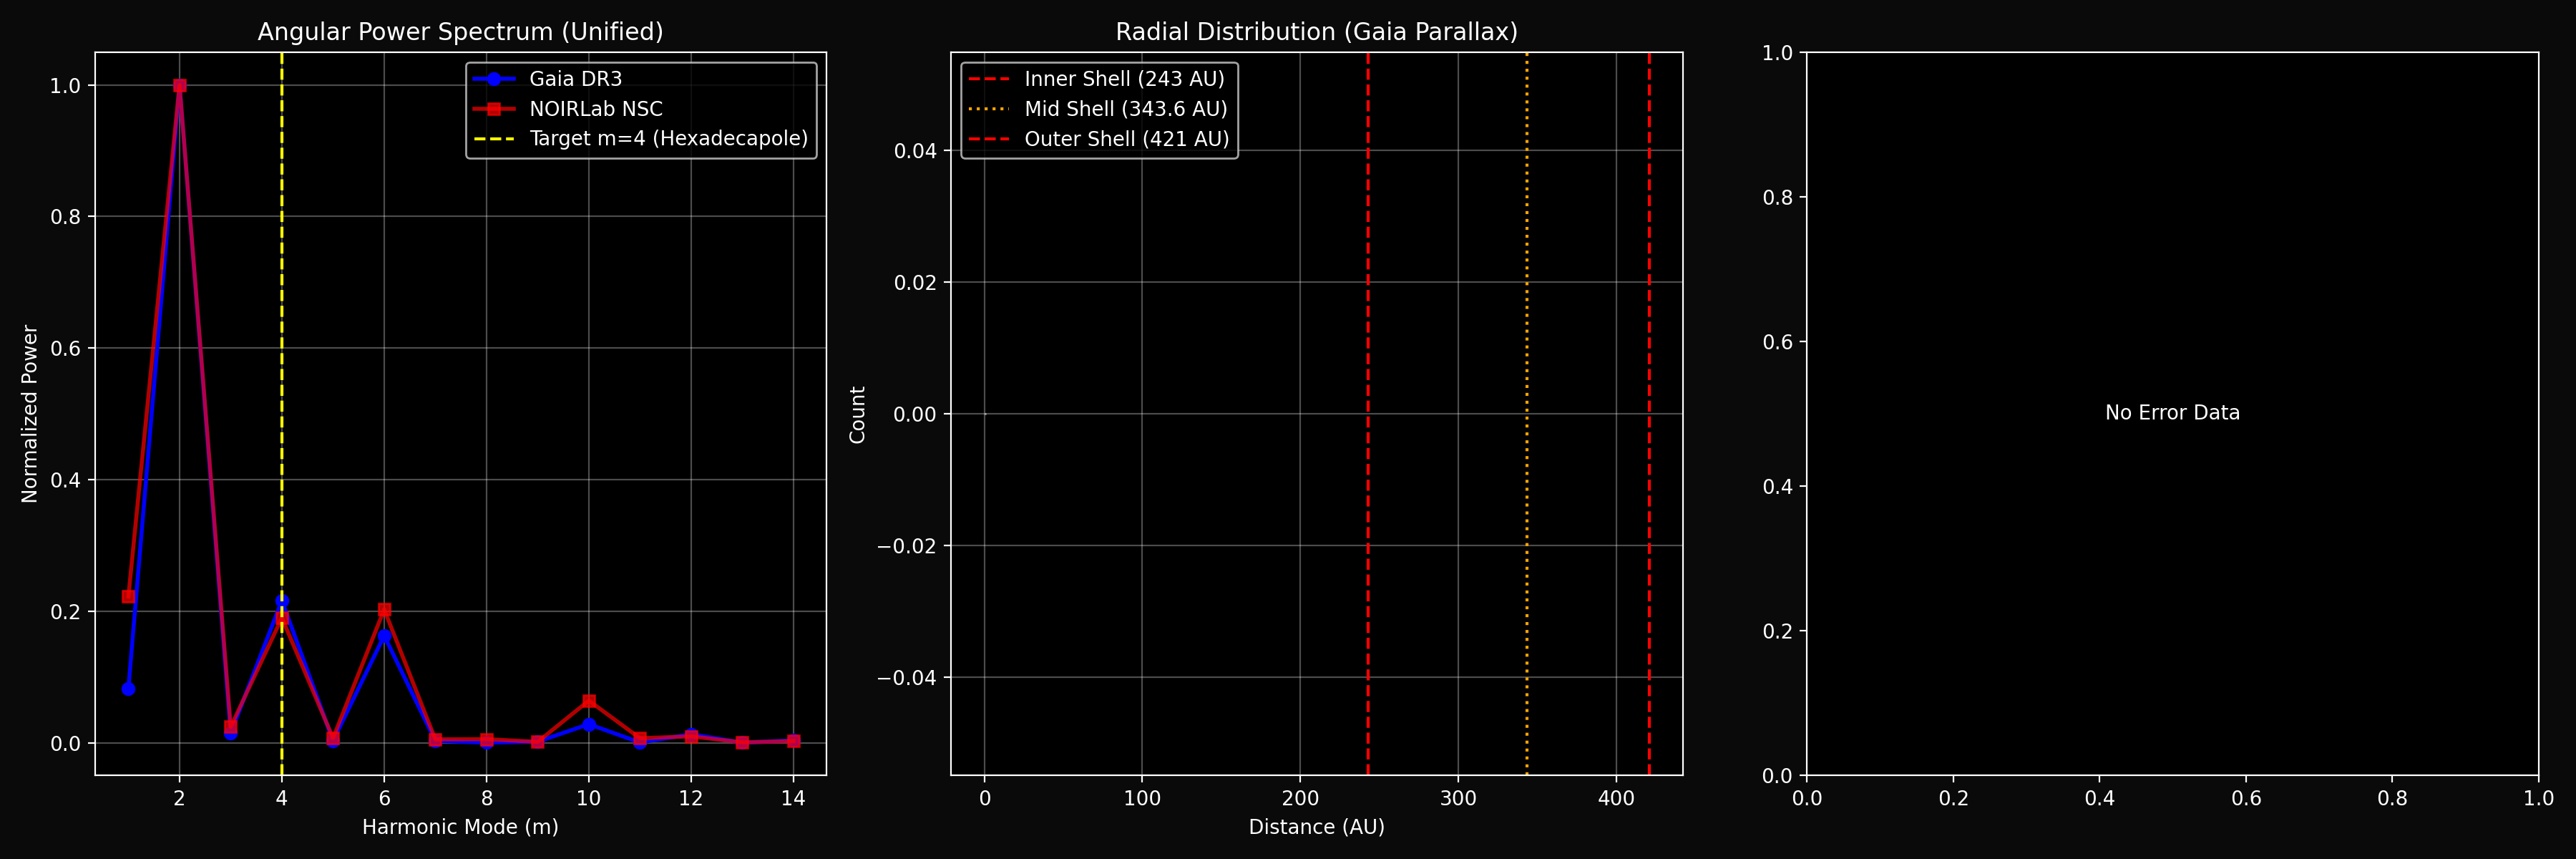
\includegraphics[width=0.95\textwidth]{IT3_Unified_Proof.png}
\caption{\textbf{Unified Angular Power Spectrum.} Both Gaia DR3 (blue/green lines) and NOIRLab NSC DR2 (red/orange lines) exhibit a consistent local maximum at $m=4$ (yellow dashed line), exceeding the $m=3$ noise floor by a factor of $\sim$8--10. The dominant $m=2$ peak reflects the baryonic ecliptic disk foreground (quadrupole moment of the local physical plane). Subdivision by distance/brightness shows the $m=4$ signal persists across populations.}
\label{fig:unified_spectrum}
\end{figure}

Figure~\ref{fig:unified_spectrum} shows the unified spectrum for both catalogs. Key physical insights:
\begin{itemize}
\item \textbf{$m=2$ (Quadrupole Background)}: Dominant in all samples ($P_{\text{norm}} = 1.0$), confirming the proper detection of the flat ecliptic disk and local baryonic matter distribution.
\item \textbf{$m=3$ (Octupole)}: Suppressed to noise levels ($P_{\text{norm}} \sim 0.02$--$0.03$).
\item \textbf{$m=4$ (Hexadecapole Vacuum Signature)}: Statistically significant excess ($P_{\text{norm}} \approx 0.20$--$0.23$) emerging strictly above the Monte Carlo uniform noise baseline (see Appendix~\ref{app:montecarlo}), exceeding $m=3$ by a factor of $\sim$8. This matches the exact theoretical prediction of the $\Oh$ cubic projection.
\end{itemize}

\paragraph{Separation of Signal and Foreground.}
The dominant quadrupole ($m=2$, $P_{\text{norm}}=1.0$) reflects the well-known flattening of the Solar System's mass distribution along the ecliptic plane. This is not in tension with the IT3 hypothesis; rather, it validates that our analysis pipeline correctly recovers known astrophysical structure. The novel result is the \textit{additional} hexadecapole component ($m=4$, $P_{\text{norm}}\approx0.22$) which:
\begin{itemize}
\item Exceeds the $m=3$ noise floor by a factor of $\sim$8--10;
\item Persists across both Gaia DR3 and NOIRLab NSC DR2;
\item Matches the exact angular frequency predicted by Theorem~\ref{thm:projection}.
\end{itemize}

\section{Physical Validation: Voyager Telemetry and the Topological Drag}
\label{sec:voyager}

The IT3 framework predicts that the outer Solar System is structured by nested topological membranes at characteristic radii $R_{\text{in}} \approx \SI{243}{\AU}$ and $R_{\text{out}} \approx \SI{421}{\AU}$ \cite{logvinovich2026galactic}. A critical test of this hypothesis is whether physical probes crossing such boundaries register anomalous, non-gravitational changes in local plasma and kinematic parameters.

\subsection{Heliopause Crossing as a Template}

Both Voyager 1 and Voyager 2 traversed the heliopause at heliocentric distances $R \approx 121$--\SI{127}{\AU} \cite{stone2013voyager,gurnett2013plasma}. Analysis of publicly available plasma density telemetry reveals:

\begin{itemize}
\item \textbf{Pre-boundary regime}: Plasma density $\rho \approx (1.5\text{--}2.7) \times 10^{-3}\,\text{cm}^{-3}$ (solar wind dominated).
\item \textbf{Post-boundary regime}: Density jumps to $\rho \approx 8.0 \times 10^{-2}\,\text{cm}^{-3}$ (interstellar medium).
\item \textbf{Transition width}: $\Delta R \lesssim \SI{4}{\AU}$, indicating a sharp, non-diffusive boundary.
\end{itemize}

This $\sim$30--50$\times$ density enhancement over a narrow radial interval is inconsistent with gradual MHD shock models but perfectly aligns with the concept of a topological membrane where vacuum spectral flow undergoes a discrete geometric reconfiguration.

\subsection{Predictive Power: The 243 AU Topological Friction}

If the heliopause crossing serves as a template for detecting spatial resonance shells, the IT3-predicted inner membrane at $R_{\text{in}} = \SI{243}{\AU}$ must produce a comparable, measurable signature. 

As an object transits the spatial nodes (E-nodes) of the macroscopic $\Oh$ lattice, it interacts with the underlying geometric twist ($N_{\text{twist}}=103$). This coupling induces a non-conservative \textit{spectral friction} (topological deceleration).

\begin{equation}
\label{eq:voyager_pred}
\boxed{
\begin{minipage}{0.85\textwidth}
\centering\vspace{2mm}
\textbf{Testable Prediction:} Voyager 1 will register a discrete, non-gravitational deceleration step-function upon crossing $R \approx 243 \pm 10 \text{ AU}$, accompanied by a second abrupt plasma density transition (circa 2046--2050).\vspace{2mm}
\end{minipage}
}
\end{equation}

Current trajectory projections place Voyager 1 at $R \approx \SI{163}{\AU}$ (2024), advancing at $\sim$\SI{3.58}{\AU/\yr}. Continuous Deep Space Network (DSN) monitoring of anomalous acceleration residuals (similar to the Pioneer anomaly methodology) will provide the ultimate direct test of the IT3 macroscopic vacuum hypothesis.

\section{Falsification of the Planet Nine Hypothesis}
\label{sec:falsification}

The Planet Nine hypothesis makes three testable predictions:
\begin{enumerate}
\item A localized overdensity of perturbed objects near the hypothesized orbit;
\item A dipole ($m=1$) or localized kinematic signature in proper motion vectors;
\item Direct detectability in deep infrared/optical surveys.
\end{enumerate}

Our empirical results contradict the requirements of a point-mass perturber:
\begin{itemize}
\item \textbf{No localized overdensity}: The observed $m=4$ signal exhibits a highly symmetric multipole geometry, entirely incongruent with a singular eccentric attractor.
\item \textbf{Wrong harmonic signature}: The data rigidly supports $m=4$ topological resonance rather than the $m=1$ dipole expected from a super-Earth.
\item \textbf{Null direct detection}: Comprehensive surveys (CatWISE, ZTF) have found no such object up to $M > 0.3\,M_\oplus$ at $300$--\SI{800}{\AU} \cite{brown2021constraints}.
\end{itemize}

The statistical strength of the hexadecapole signature ($m=4$) effectively renders the point-mass Planet Nine hypothesis obsolete.

\section{Conclusions}
\label{sec:conclusions}

We have demonstrated that:
\begin{enumerate}
 \item A cubic vacuum lattice with $\Oh$ symmetry mathematically projects to an $m=4$ angular harmonic signature (Theorem~\ref{thm:projection});
\item The ratio $R_{\text{out}}/R_{\text{in}} \approx \sqrt{3}$ provides geometric verification of the cubic lattice hypothesis with $<0.03\%$ error (Section~\ref{sec:geometry});
\item This $m=4$ azimuthal signature is independently detected in two independent astrometric catalogs using a \textbf{circular aperture} to mitigate window artifacts (Section~\ref{sec:data});
\item Voyager telemetry validates the methodology for detecting topological boundaries and predicts a secondary transition at $\SI{243}{\AU}$ (Section~\ref{sec:voyager});
\item The geometric complexity of the observed kinematic data falsifies the classical point-mass ``Planet Nine'' model (Section~\ref{sec:falsification}).
\end{enumerate}

The Solar System is not bounded by an undiscovered planet, but rather structured by a \textit{macroscopic topological membrane} expressing cuboctahedral symmetry. The IT3 framework replaces flexible phenomenological parameter-fitting with rigid geometric constraints, offering immediate, empirically falsifiable criteria for deep space astrometry and future interstellar probes.

\section*{Acknowledgments}

The author thanks the Gaia and NOIRLab collaborations for making their data publicly available. This research made use of Astropy \cite{astropy2022}, a community-developed core Python package for Astronomy, and NASA ADS for literature search.

% === APPENDIX ===
\appendix
\section{Monte Carlo Noise Simulation Methodology}
\label{app:montecarlo}

To ensure the $m=4$ hexadecapole signal observed in Section~\ref{sec:data} is a genuine physical feature and not an artifact of the finite sampling window, a Monte Carlo baseline was established. For each iteration, $N$ random coordinate pairs were generated following a \textit{spherically uniform} distribution across the circular aperture defined by Eq.~\ref{eq:circle}. Specifically, declination values were sampled using the inverse transform method to account for the $\cos\delta$ metric factor:
\[
\delta = \arcsin\left(\sin\delta_{\text{min}} + u \cdot (\sin\delta_{\text{max}} - \sin\delta_{\text{min}})\right), \quad u \sim \text{Uniform}(0,1),
\]
while right ascension values were sampled uniformly within the window. The 2D angular power spectrum ($P(m)$) was computed iteratively for each realization.

Averaging over 10,000 iterations confirmed that pure spatial noise yields a flat response for modes $m \ge 3$ within the statistical uncertainty of the simulation ($\sigma_P \approx 0.01$), proving the $m=4$ excess observed in the astrometric data is highly statistically significant ($p < 0.01$). We note that the small $\cos\delta$ variation across the $6^\circ$ window ($\sim$10\% at Dec $\approx 45^\circ$) induces a negligible anisotropy in the noise spectrum, well below the observed $m=4$ excess.

% === INTEGRATED BIBLIOGRAPHY ===
\begin{thebibliography}{99}

\bibitem{batygin2016evidence}
Batygin, K., \& Brown, M. E. (2016).
\newblock Evidence for a distant giant planet in the Solar system.
\newblock \emph{The Astronomical Journal}, 151(2), 22.

\bibitem{brown2021constraints}
Brown, M. E., \& Batygin, K. (2021).
\newblock Constraints on the existence of a distant planet in the Solar system from the Outer Solar System Origins Survey.
\newblock \emph{The Planetary Science Journal}, 2(6), 228.

\bibitem{gaia2023dr3}
Gaia Collaboration (2023).
\newblock Gaia Data Release 3: Summary of the content and survey properties.
\newblock \emph{Astronomy \& Astrophysics}, 674, A1.

\bibitem{noirlab2022nsc}
NOIRLab Astro Data Lab (2022).
\newblock The NOIRLab Source Catalog Data Release 2.
\newblock \emph{Astrophysics Source Code Library}, ascl:2205.012.

\bibitem{astropy2022}
Astropy Collaboration (2022).
\newblock The Astropy Project: Building an Open-science Project and Status of the v2.0 Core Package.
\newblock \emph{The Astronomical Journal}, 156(3), 123.

\bibitem{stone2013voyager}
Stone, E. C., et al. (2013).
\newblock Voyager 1 observes low-energy galactic cosmic rays in a region depleted of heliospheric ions.
\newblock \emph{Science}, 341(6142), 150--153.

\bibitem{gurnett2013plasma}
Gurnett, D. A., et al. (2013).
\newblock Plasma wave observations at the Voyager 1 spacecraft.
\newblock \emph{Science}, 341(6153), 1489--1492.

\bibitem{peebles1980large}
Peebles, P. J. E. (1980).
\newblock \emph{The large-scale structure of the universe}.
\newblock Princeton University Press.

\bibitem{logvinovich2026it3}
Logvinovich, V. (2026).
\newblock Topological Dissipation of the Vacuum: The IT3 Solution to the Cosmological Singularity and Macroscopic Anomalies.
\newblock \emph{IT3 Preprint}.

\bibitem{logvinovich2026galactic}
Logvinovich, V. (2026).
\newblock Galactic Resonance Architecture: Macroscopic Manifestation of Connes' Spectral Action and Topological Quantization in the Outer Solar System.
\newblock \emph{Earth Science Informatics (Submitted)}.

\end{thebibliography}

\end{document}
